\chapter{Liquid water production in martian impacts}
\label{ch04}

Observations by HiRise\footnote{High Resolution Imaging Science Experiment: \url{http://hirise.lpl.arizona.edu/}} lead to the discovery of several fresh impact crater sites on Mars with relatively blue appearing material on the crater bottoms. Follow-up observations of the crater bottoms with the Context Imager (CTX) onboard the Mars Reconnaissance Orbiter and optical spectra provided by CRISM\footnote{Compact Reconnaissance Imaging Spectrometer for Mars: \url{http://crism.jhuapl.edu}} unambiguously associated the observations to water ice. 
The relatively clean surfaces of those icy crater bottoms raised questions about their formation mechanism. A normal cratering event would have  left debris in the form of shattered ice and surface soils on the crater bottom, but not a clean surface. The main question addressed in the following paper was, whether a sub-surface ice layer could have undergone strong enough shock-heating during the impact to undergo a phase change and produce liquid water.  

We used a solid SPH code with a fracture model, to simulate impact scenarios which lead to the observed crater sizes and analyzed the peak shock pressures reached in the water ice layer. Thermodynamic data from shock experiments allowed us to estimate the amount of ice undergoing phase changes, simply due to shock heating. We found that depending on the assumed soil layer and the impact parameters, up to several $100 kg$ can be produced during such impact events.

\includepdf[pages={2-},fitpaper=true]{04figs/f9d1219a0fca0f2cd983b857ca6e3705.pdf}